% Section 7: Results (SCOPAS dual-layer revision)
% Numbers below are from paper_rerun_city_dual / run_medium (see MANIFEST.md).
% Replace airport / Paulista placeholders once those runs complete.

\section{Results and Analysis}
\label{sec:results}

We report dual-layer NSGA-II fronts under SCOPAS: maximize threat-weighted cooperative coverage \(M_{wp,coop}\) and non-cooperative coverage \(M_{wp,noncoop}\) while minimizing CapEx (hardware + site activation). Non-cooperative sensors are Radar, EO, and Acoustic; RF contributes only to the cooperative layer.

\subsection{Synthetic city (1\,km$\times$1\,km, five critical assets)}

Configuration: resolution 30\,m, population 32, 18 generations, 4 cores, sensor budget 3--15, Acoustic enabled. The run produced 32 non-dominated solutions. Cooperative coverage spans \(0.074\)--\(0.963\); non-cooperative coverage spans \(0.003\)--\(0.563\).

\begin{figure}[t]
  \centering
  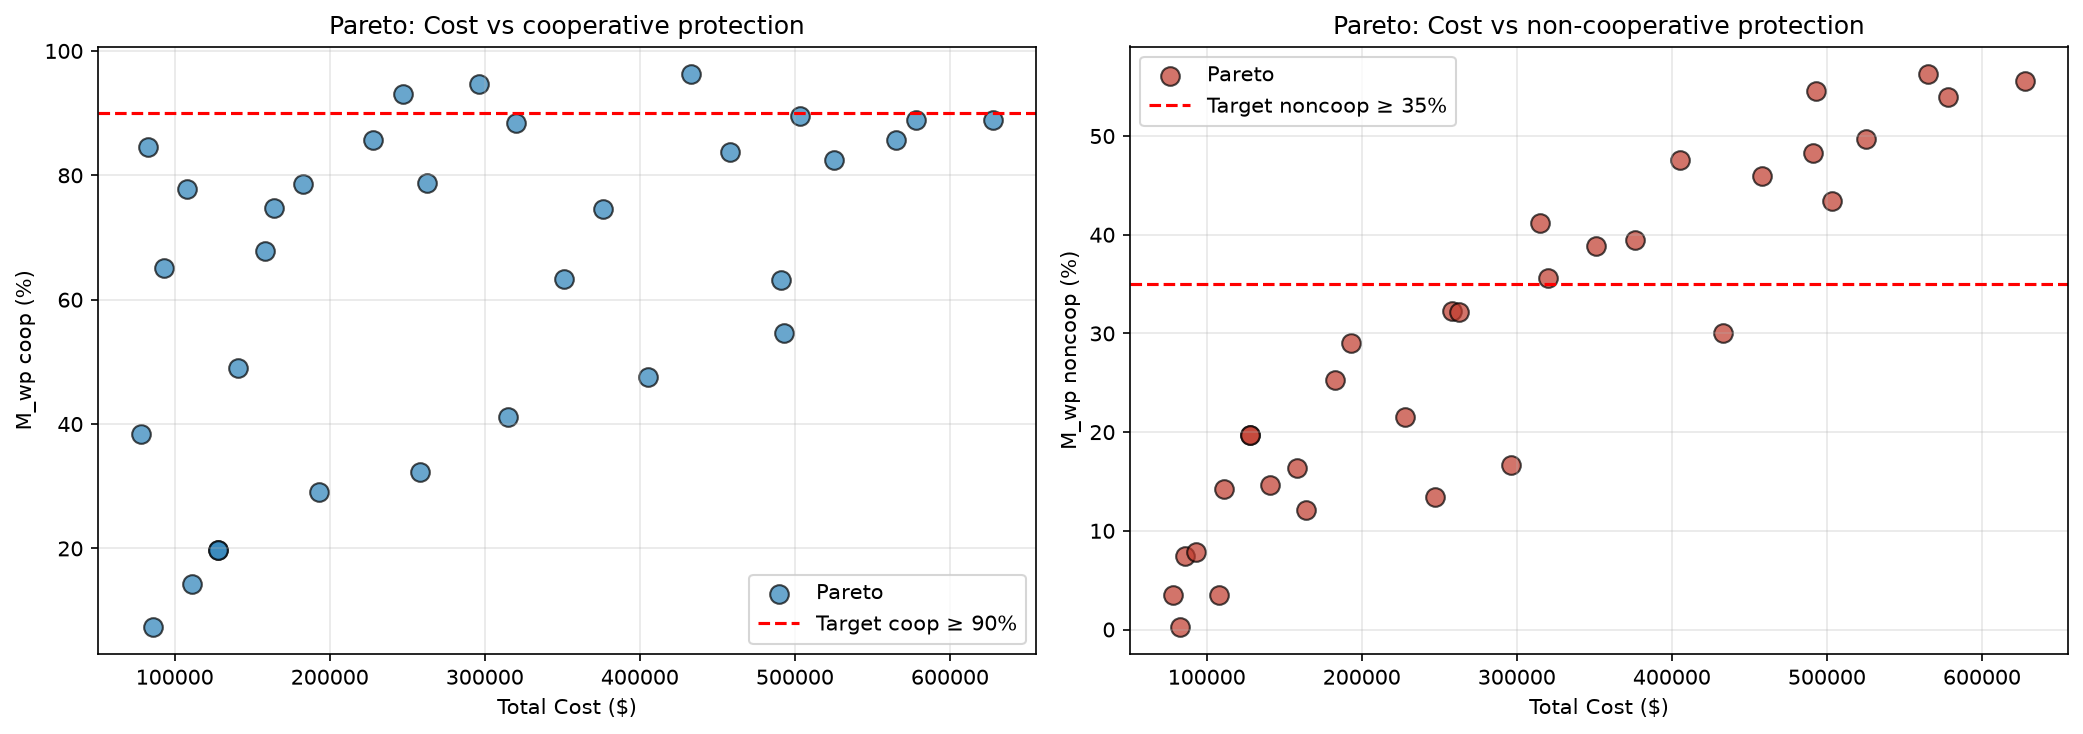
\includegraphics[width=0.48\textwidth]{figures/scopas/city_pareto_front.png}
  \caption{Dual-layer Pareto projections for the synthetic city (cost vs.\ \(M_{wp,coop}\) and \(M_{wp,noncoop}\)).}
  \label{fig:city_pareto}
\end{figure}

\begin{figure}[t]
  \centering
  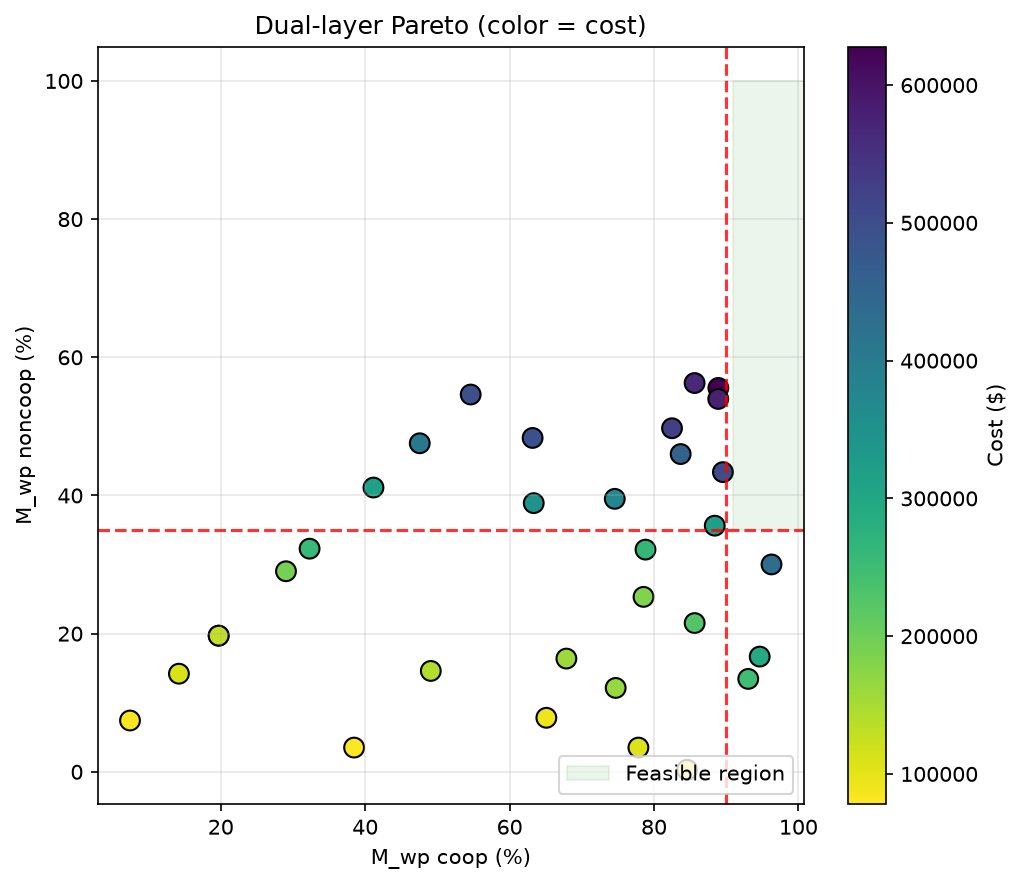
\includegraphics[width=0.48\textwidth]{figures/scopas/city_dual_targets.png}
  \caption{Coop$\times$noncoop trade space with planning floors \(M_{wp,coop}\geq0.90\) and \(M_{wp,noncoop}\geq0.35\) (green box). Color encodes CapEx.}
  \label{fig:city_targets}
\end{figure}

\subsubsection{Representative operating points}

\begin{table}[h]
\centering
\caption{Representative dual-layer solutions — synthetic city (SCOPAS rerun).}
\label{tab:city_dual}
\begin{tabular}{lcccc}
\toprule
\textbf{Regime} & \textbf{Mix} & \(M_{wp,coop}\) & \(M_{wp,noncoop}\) & \textbf{Cost} \\
\midrule
Cheap coop & 2RF+1Ac & 0.846 & 0.003 & \$83k \\
Joint near-floor & 4Rad+2RF & 0.884 & 0.356 & \$320k \\
High coop & 4Rad+5RF+1Ac & 0.963 & 0.300 & \$433k \\
Best joint miss & 6Rad+3RF+1Ac & 0.895 & 0.434 & \$503k \\
Best noncoop & 7Rad+2EO+1RF & 0.856 & 0.563 & \$565k \\
\bottomrule
\end{tabular}
\end{table}

\textbf{Finding 1 (layer asymmetry).}
Cooperative coverage \(\geq90\%\) is reachable near \$247k, but that individual only achieves \(M_{wp,noncoop}=0.134\). Dark-target coverage above \(0.50\) requires Radar-heavy mixes above \$500k and still does not jointly clear a strict \(0.90/0.50\) box in this budget.

\textbf{Finding 2 (practical joint floor).}
Under floors \(0.90/0.35\), the front has no feasible member (closest: \(0.895/0.434\) at \$503k). Softening to \(0.85/0.35\) yields five feasible solutions; cheapest \$320k (4 Radar + 2 RF). Stretch demos on the same geometry previously found a joint \(0.90/0.35\) solution at \$315k with a larger dual-layer search (see \texttt{demo\_targets} package).

\textbf{Finding 3 (altitude still matters).}
Flight-level analysis preserves the airway gap narrative: low airways remain occlusion-limited even when aggregate \(M_{wp}\) is high (Figure~\ref{fig:city_flight}).

\begin{figure}[t]
  \centering
  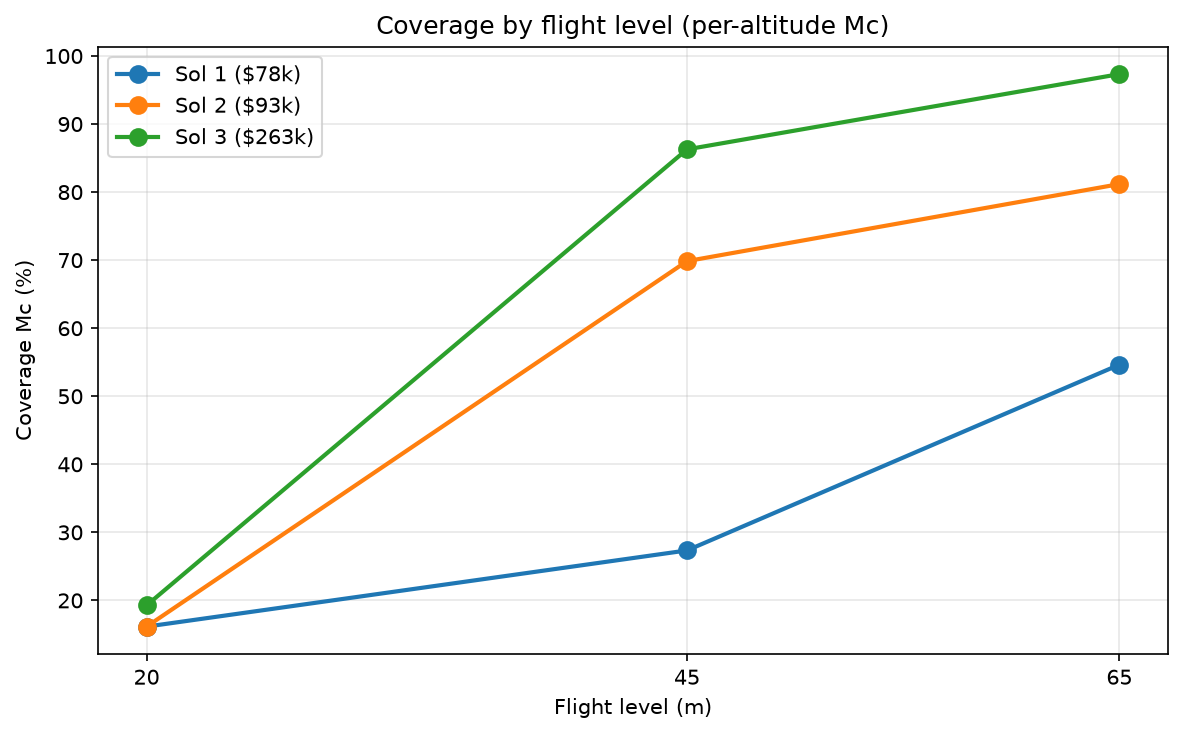
\includegraphics[width=0.48\textwidth]{figures/scopas/city_flight_levels.png}
  \caption{Coverage by flight level for representative Pareto members.}
  \label{fig:city_flight}
\end{figure}

\begin{figure}[t]
  \centering
  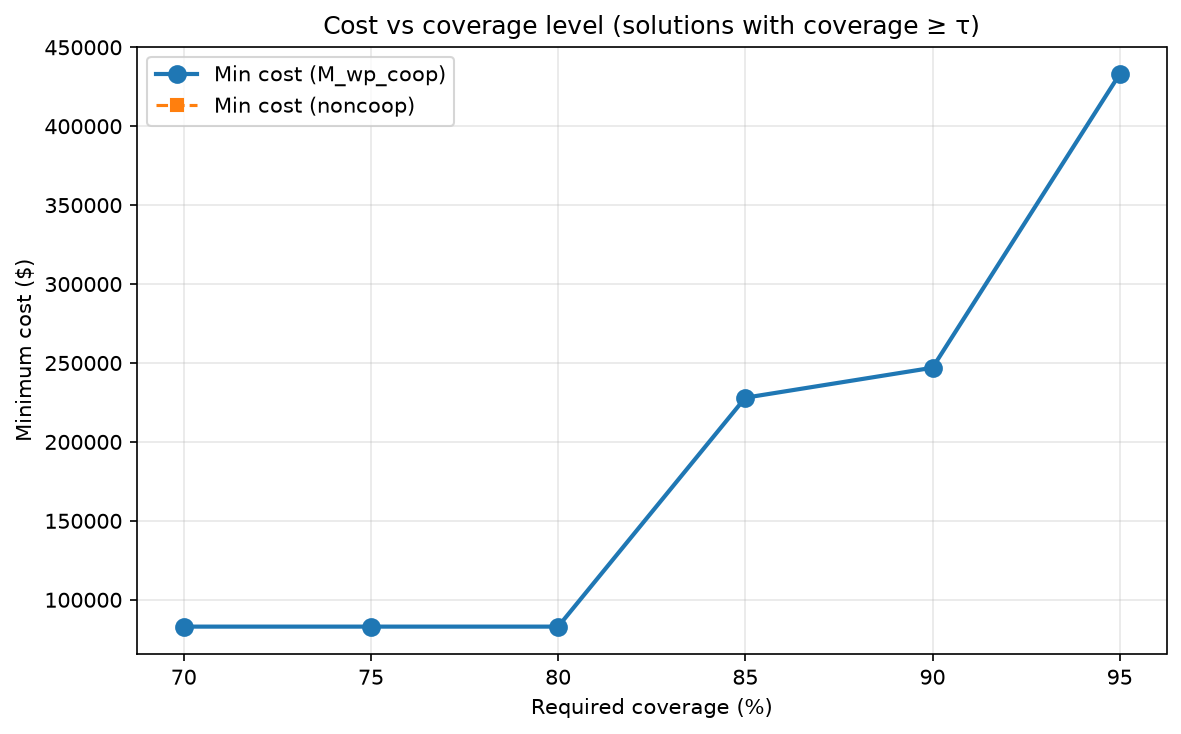
\includegraphics[width=0.48\textwidth]{figures/scopas/city_cost_vs_coverage.png}
  \caption{Minimum CapEx to reach cooperative \(M_{wp}\) thresholds; non-cooperative 70\%+ thresholds remain empty on this front.}
  \label{fig:city_cost_thr}
\end{figure}

\subsection{Requirement-seeking demos (prior short runs)}

Target-seeking configs aiming at \(0.90/0.35\) and stretch \(0.90/0.50\) confirm the same structure: cooperative floors are inexpensive with RF; joint dark-target floors near \(35\%\) are the practical planning corridor; \(50\%\) noncoop with \(\geq90\%\) coop remains a stretch (best observed joint near \(0.957/0.445\)).

\subsection{Airport SJC split fronts}

Split optimization on the São José dos Campos airport scene (resolution 40\,m, population 24, 12 generations) isolates each layer.

\textbf{Cooperative front.} Twenty-four solutions; \(M_{wp,coop}\) saturates to \(1.0\). The cheapest plan with \(M_{wp,coop}\geq0.90\) costs \$61k (1 RF + 2 Acoustic) but yields \(M_{wp,noncoop}\approx0.004\). High-coop RF-heavy plans at \$188k still leave non-cooperative coverage near zero.

\textbf{Non-cooperative front.} Twenty-four Radar/EO/Acoustic solutions span \(M_{wp,noncoop}\) from \(0.032\) to \(0.445\). Best observed dark-target coverage is \(0.445\) at \$405k (5 Radar + 2 EO); no plan reaches a 70\% noncoop threshold in this budget.

\begin{figure}[t]
  \centering
  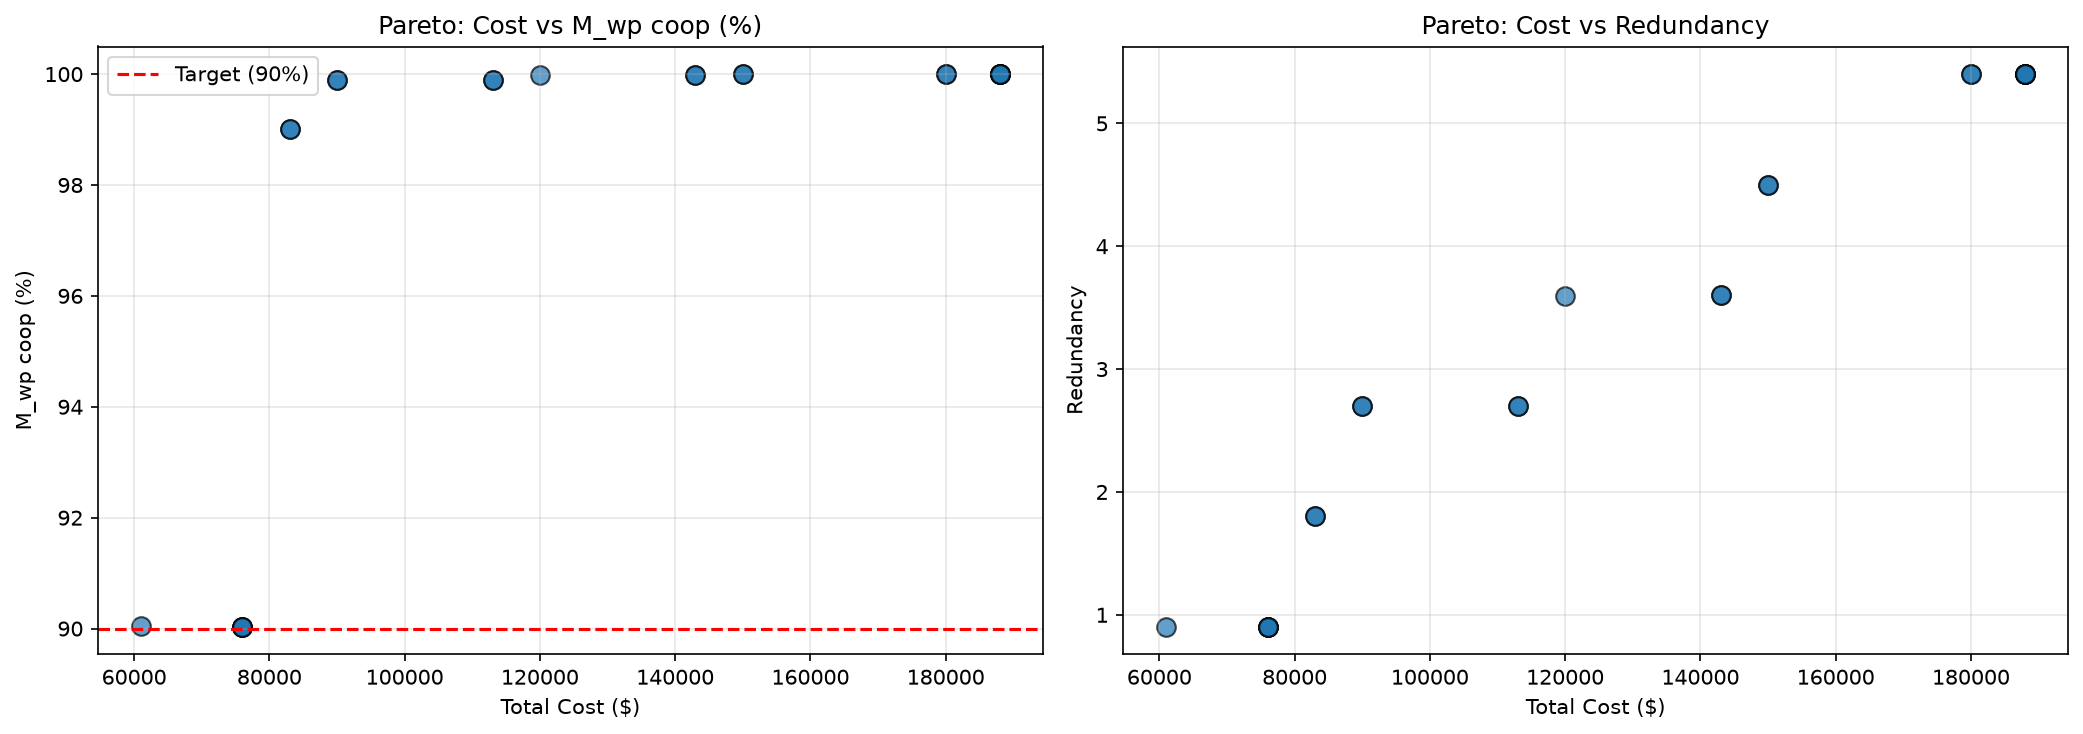
\includegraphics[width=0.48\textwidth]{figures/scopas/sjc_coop_pareto.png}
  \caption{Airport SJC cooperative-only Pareto (cost vs.\ \(M_{wp,coop}\)).}
  \label{fig:sjc_coop}
\end{figure}

\begin{figure}[t]
  \centering
  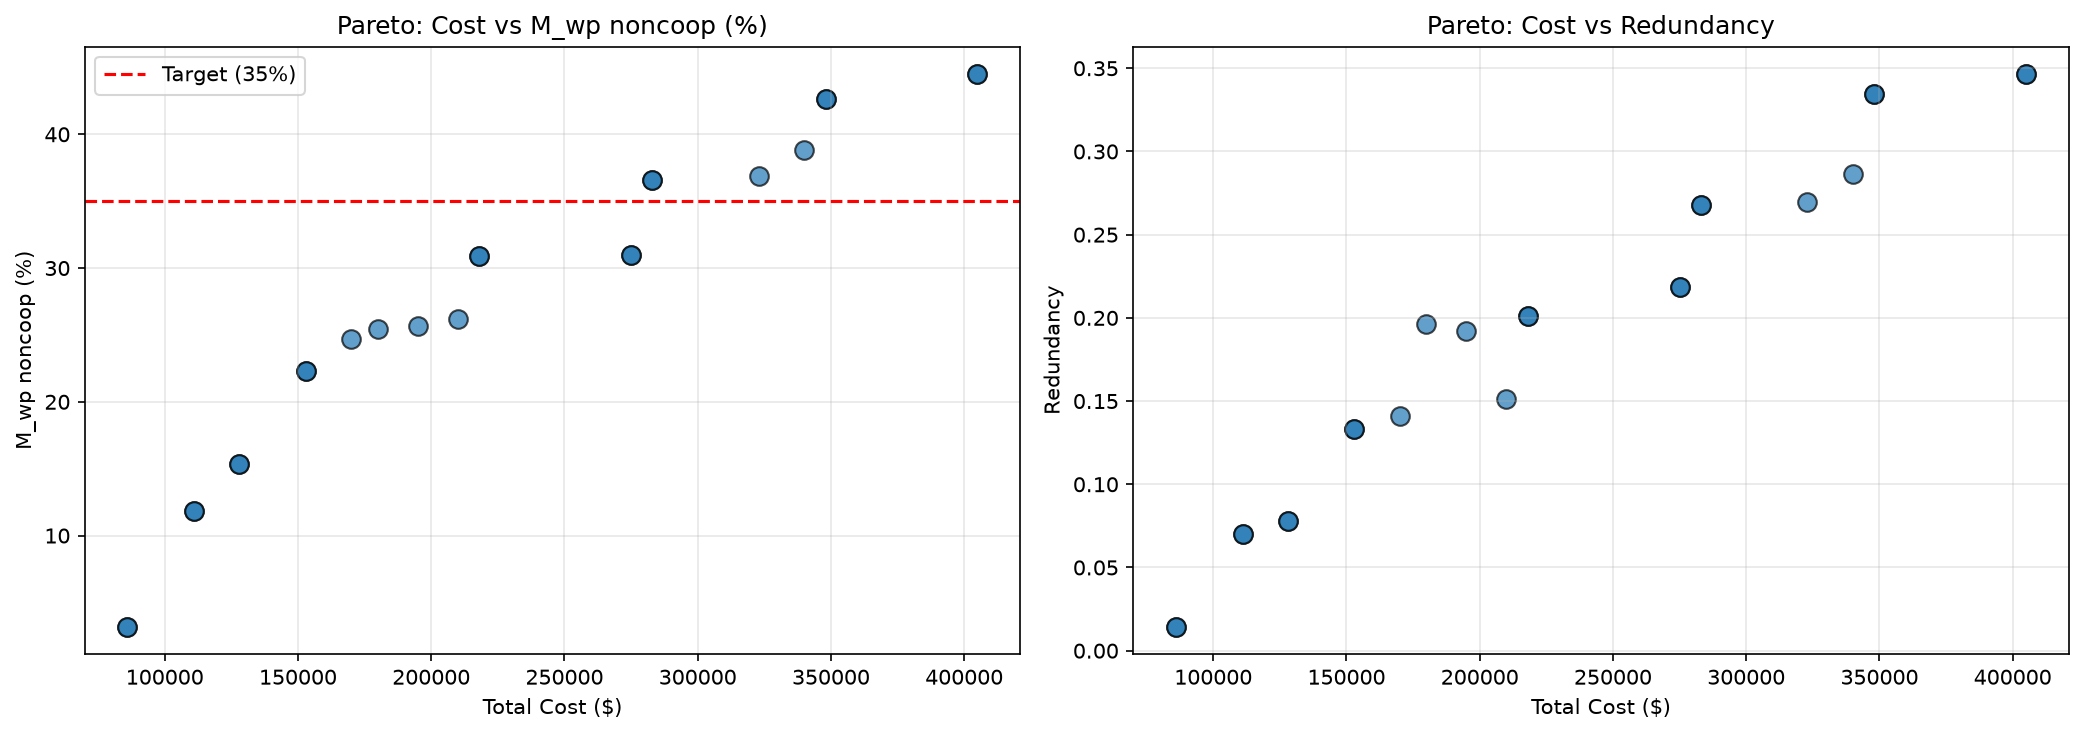
\includegraphics[width=0.48\textwidth]{figures/scopas/sjc_noncoop_pareto.png}
  \caption{Airport SJC non-cooperative-only Pareto (cost vs.\ \(M_{wp,noncoop}\)).}
  \label{fig:sjc_noncoop}
\end{figure}

This split is the operational punchline: a cooperative optimum is \emph{not} a dark-target plan. BVLOS safety cases that quote a single coverage percentage from RF-inclusive optimization overstate non-cooperative protection.

\subsection{Avenida Paulista lite}

Lite dual-layer rerun of the prior real-city case (6,389 buildings, 93 sites, resolution 40\,m, population 24, 10 generations) produced 24 solutions. Cooperative coverage reaches \(0.970\) (\$311k, RF-heavy mix); non-cooperative coverage tops out at \(0.254\) (\$464k, Radar-heavy). No joint member meets even \(0.85/0.25\) in this budget (closest deficits remain on the noncoop axis).

\begin{figure}[t]
  \centering
  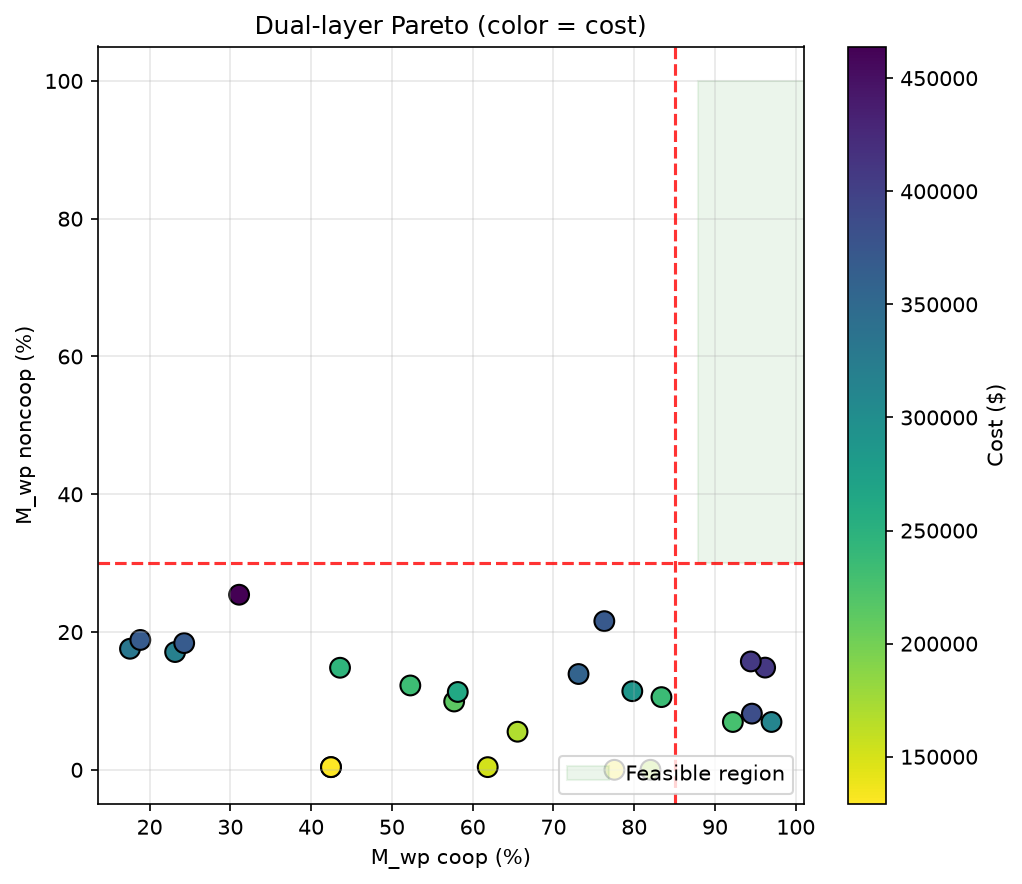
\includegraphics[width=0.48\textwidth]{figures/scopas/paulista_targets.png}
  \caption{Paulista lite dual-layer trade space (color = CapEx).}
  \label{fig:paulista_targets}
\end{figure}

Relative to the synthetic city, the dense corridor compresses dark-target performance harder than cooperative RID coverage --- reinforcing that Paulista-class canyons need either denser noncoop deployments, relaxed floors, or altitude policy, not merely more RF nodes.

Full paper-budget Paulista (80$\times$45 @ 20\,m) remains a longer checkpointed job for the camera-ready revision.

\subsection{Control A: small-$n$ oracle vs.\ GA}
\label{sec:results_oracle}

Table~\ref{tab:oracle_comparison} reports Control~A under the protocol of Section~\ref{sec:protocol_oracle}. On fully enumerable instances (\(n{=}8,k{=}3\) and \(n{=}10,k{=}4\)), NSGA-II* matches the oracle \(M_c\) exactly (\(\Delta{=}0.0\)\,pp). At \(n{=}12,k{=}5\) (type-sampled oracle), the gap is \(0.3\)\,pp. Greedy is competitive; Random trails on the largest crop. Wall-clock for the oracle stays under a few seconds at this resolution because \(P_D\) grids are precomputed.

\textbf{Interpretation.} Where exhaustive search is feasible, the GA recovers near-oracle classic \(M_c\) under the same ray-tracer. We treat this as method validation on enumerable instances---\emph{not} as a city-scale optimality certificate for dual-layer fronts with \(n\gtrsim25\).

\begin{table}[t]
\centering
\caption{Control A — small-$n$ oracle. $\Delta M_c$ = oracle $-$ method (same ray-tracer). NSGA-II* is a fixed-$k$ $M_c$-maximizing GA (5 seeds).}
\label{tab:oracle_comparison}
\begin{tabular}{ccrrrrrr}
\toprule
$n$ & $k$ & Oracle $M_c$ & Greedy & Random & NSGA-II* & $\Delta_{\mathrm{NSGA}}$ & $t_{\mathrm{oracle}}$ (s) \\
\midrule
8 & 3 & 89.1\% & 89.1\% & 89.1\% & 89.1\% & 0.0\,pp & 0.1 \\
10 & 4 & 91.5\% & 91.5\% & 91.2\% & 91.5\% & 0.0\,pp & 1.5 \\
12 & 5 & 96.2\% & 95.9\% & 92.7\% & 95.9\% & 0.3\,pp & 2.0 \\
\bottomrule
\end{tabular}
\end{table}


\subsection{Control B: matched CapEx modality ablation}
\label{sec:results_ablation}

Table~\ref{tab:modality_ablation} reports best classic \(M_c\) at three CapEx budgets. RF-only wins at \$31k (\(88.3\%\) vs.\ heterogeneous \(82.3\%\)) and \$76k (\(95.3\%\) vs.\ \(93.8\%\)). Heterogeneous only edges RF at \$150k (\(98.3\%\) vs.\ \(98.0\%\)). Acoustic-only and EO-only remain near zero / single-digit \(M_c\) at these budgets (short effective range under the \(0.8\) threshold); Radar-only is infeasible at \$31k and weak thereafter relative to RF for classic coverage.

\textbf{Interpretation.} For CapEx-matched classic \(M_c\), heterogeneity is \emph{not} universally superior: lean and mid budgets favor RF-dominant layouts. Heterogeneity becomes competitive only at higher CapEx. This softens any ``always heterogeneous'' claim. Dual-layer airport splits still show why RF-only plans fail dark-target floors---the modality story depends on whether the planning metric is cooperative \(M_c\) or joint coop/noncoop.

\begin{table}[t]
\centering
\caption{Control B — matched CapEx modality ablation (hardware only). Best $M_c$ under each budget.}
\label{tab:modality_ablation}
\begin{tabular}{lrrrrr}
\toprule
Budget & RF-only & Ac-only & EO-only & Radar-only & Heterogeneous \\
\midrule
\$31k & 88.3\% & 0.0\% & 0.9\% & --- & 82.3\% \\
\$76k & 95.3\% & 0.0\% & 2.9\% & 5.1\% & 93.8\% \\
\$150k & 98.0\% & 0.0\% & 5.2\% & 14.2\% & \textbf{98.3\%} \\
\bottomrule
\end{tabular}
\end{table}


\subsection{Control C: dual-layer CapEx ablation}
\label{sec:results_dual_ablation}

Tables~\ref{tab:modality_ablation_dual_coop}--\ref{tab:modality_ablation_dual_noncoop} report Control~C. On the cooperative axis, RF-only wins every budget (\$31k--\$320k) with \(M_{wp,coop}\) from \(89.3\%\) to \(99.6\%\), but companion noncoop stays at \(0\%\). On the non-cooperative axis, EO-only leads at \$31k/\$76k (\(7.2\%\)/\(17.2\%\)); Radar-only leads at \$150k (\(33.7\%\), matched by a Radar-heavy heterogeneous pack); Heterogeneous wins at \$320k with \(M_{wp,noncoop}=47.5\%\) and companion coop \(82.6\%\).

\textbf{Interpretation.} Dual-layer CapEx matching overturns any RF-only reading of Control~B: RF saturates coop while contributing nothing to dark targets. Heterogeneity is \emph{necessary for joint floors} near the \$320k band, not for lean classic \(M_c\). Lean noncoop budgets favor dense EO/Acoustic fills over mixed packs; mixed Radar/RF/EO/Acoustic wins when both layers must be high together.

\begin{table}[t]
\centering
\caption{Control C — dual-layer CapEx ablation. Best $M_{wp,\mathrm{coop}}$ under each hardware budget (companion $M_{wp,\mathrm{noncoop}}$ in parentheses).}
\label{tab:modality_ablation_dual_coop}
\begin{tabular}{lrrrrr}
\toprule
Budget & RF-only & Ac-only & EO-only & Radar-only & Heterogeneous \\
\midrule
\$31k & 89.3\% (0\%) & 3.9\% (4\%) & 7.2\% (7\%) & --- & 76.8\% (2\%) \\
\$76k & 95.3\% (0\%) & 9.1\% (9\%) & 17.2\% (17\%) & 14.0\% (14\%) & 94.6\% (1\%) \\
\$150k & 98.4\% (0\%) & 13.4\% (13\%) & 23.7\% (24\%) & 33.7\% (34\%) & 98.4\% (0\%) \\
\$320k & 99.6\% (0\%) & 13.4\% (13\%) & 39.5\% (40\%) & 43.8\% (44\%) & 98.7\% (23\%) \\
\bottomrule
\end{tabular}
\end{table}

\begin{table}[t]
\centering
\caption{Control C — dual-layer CapEx ablation. Best $M_{wp,\mathrm{noncoop}}$ under each hardware budget (companion $M_{wp,\mathrm{coop}}$ in parentheses).}
\label{tab:modality_ablation_dual_noncoop}
\begin{tabular}{lrrrrr}
\toprule
Budget & RF-only & Ac-only & EO-only & Radar-only & Heterogeneous \\
\midrule
\$31k & 0.0\% (89\%) & 3.9\% (4\%) & 7.2\% (7\%) & --- & 3.1\% (23\%) \\
\$76k & 0.0\% (95\%) & 9.1\% (9\%) & 17.2\% (17\%) & 14.0\% (14\%) & 3.1\% (92\%) \\
\$150k & 0.0\% (98\%) & 13.4\% (13\%) & 23.7\% (24\%) & 33.7\% (34\%) & 33.7\% (34\%) \\
\$320k & 0.0\% (100\%) & 13.4\% (13\%) & 39.5\% (40\%) & 43.8\% (44\%) & \textbf{47.5\% (83\%)} \\
\bottomrule
\end{tabular}
\end{table}

